%% ============================================================
%%  Traffic Object Detection, Tracking and Safety Analysis
%%  B.Tech Project Thesis
%%
%%  Main driver file — \includes all chapter files.
%%  Follows the structural and package conventions of the
%%  professor's report.md template (pkmthesis-compatible).
%%
%%  To compile:
%%    1. pdflatex thesis.tex
%%    2. bibtex thesis
%%    3. pdflatex thesis.tex
%%    4. pdflatex thesis.tex
%% ============================================================

\documentclass[12pt,a4paper]{report}

%% ---- Packages (identical to report.md preamble) ----
\usepackage{amsmath,amssymb,epsfig,graphicx,setspace,url,float}
\usepackage{lscape,multicol,multirow,longtable,subfigure}
\usepackage{cite,bm}
\usepackage{geometry}
\usepackage{array}
\usepackage{algorithm}
\usepackage{algpseudocode}
\usepackage{multirow}
\usepackage{tabularx}
\usepackage{subcaption}
\usepackage{booktabs}
\usepackage[english]{babel}
\usepackage[small,bf]{caption}
\usepackage{csquotes}
\usepackage{threeparttable}
\usepackage{xcolor}
\usepackage{fancyhdr}
\usepackage{hyperref}
\usepackage{listings}
\usepackage{tikz}
\usepackage{pgfplots}
\pgfplotsset{compat=1.18}

%% ---- Page layout ----
\geometry{a4paper, top=2.5cm, bottom=2.5cm, left=3.5cm, right=2.5cm, headheight=15pt}
\setlength{\abovecaptionskip}{8pt}
\setlength{\belowcaptionskip}{8pt}
\setlength{\textfloatsep}{1cm}
\raggedbottom

%% ---- hyperref ----
\hypersetup{
  colorlinks=true, linkcolor=blue, citecolor=blue, urlcolor=blue,
  pdftitle={Traffic Object Detection, Tracking and Safety Analysis},
  pdfauthor={K. Narain Varma}
}

%% ---- Listings ----
\lstset{basicstyle=\ttfamily\small,breaklines=true,frame=single,
        keywordstyle=\color{blue}\bfseries,commentstyle=\color{gray},
        stringstyle=\color{red!70!black},numbers=left,
        numberstyle=\tiny\color{gray},tabsize=4,showstringspaces=false}

%% ===========================================================
\begin{document}

\setcounter{page}{1}
\pagenumbering{roman}
\doublespacing

%% ---- Title page -------------------------------------------
\begin{titlepage}
\thispagestyle{empty}
\begin{center}
    \vspace*{0.5cm}
    {\Large\bfseries Traffic Object Detection, Tracking, and Automated Safety\\
    Analysis at an Indian Roundabout Intersection}\\[2cm]
    {\large A B.Tech Project Report submitted in partial fulfilment of the requirements
    for the degree of Bachelor of Technology}\\[1.5cm]
    {\large by}\\[0.5cm]
    {\Large\bfseries K. Narain Varma}\\[0.3cm]
    {\large Roll No.\ [TO BE FILLED]}\\[2cm]
    {\large Under the Supervision of}\\[0.5cm]
    {\Large\bfseries [Supervisor Name]}\\[0.3cm]
    {\large [Designation]}\\[2cm]
    \vfill
    {\large\bfseries Department of [Department Name]}\\[0.3cm]
    {\large [Institute Name]}\\[0.5cm]
    {\large [City, State, India]}\\[0.3cm]
    {\large [Month and Year]}
\end{center}
\end{titlepage}
\clearpage\thispagestyle{empty}

%% ---- Certificate ------------------------------------------
\newpage\thispagestyle{empty}
\chapter*{Certificate}
\addcontentsline{toc}{chapter}{Certificate}
\vspace{1cm}

This is to certify that the project titled \textbf{``Traffic Object Detection, Tracking,
and Automated Safety Analysis at an Indian Roundabout Intersection''} submitted by
\textbf{K. Narain Varma} (Roll No.\ [TO BE FILLED]) in partial fulfilment of the
requirements for the award of the Degree of \textbf{Bachelor of Technology} is a record of
bonafide work carried out by the student under our supervision in the Department of
[Department Name], [Institute Name].

\vspace{2cm}
\noindent
\begin{tabular}{p{7cm}p{7cm}}
\textbf{[Supervisor Name]} & \textbf{[HOD Name]}\\
{[Designation]}            & Head, Dept.\ of [Department Name]\\
{[Institute Name]}         & [Institute Name]\\
{[City, India]}            & [City, India]\\
\end{tabular}

\clearpage\thispagestyle{empty}

%% ---- Declaration ------------------------------------------
\newpage\thispagestyle{empty}
\chapter*{Declaration}
\addcontentsline{toc}{chapter}{Declaration}

\noindent
I, \textbf{K. Narain Varma}, hereby declare that the project report entitled
\textbf{``Traffic Object Detection, Tracking, and Automated Safety Analysis at an Indian
Roundabout Intersection''}, submitted in partial fulfilment of the requirements for the
award of the degree of Bachelor of Technology, is my own work and has not been submitted
elsewhere for the award of any degree or diploma.

\vspace{2cm}
\noindent
\textbf{K. Narain Varma}\\
Roll No.\ [TO BE FILLED]\\
[Date]

\clearpage\thispagestyle{empty}

%% ---- Acknowledgement --------------------------------------
\newpage\thispagestyle{empty}
\chapter*{Acknowledgement}
\addcontentsline{toc}{chapter}{Acknowledgement}

\noindent
[Acknowledgement text to be filled by the student.]

\clearpage\thispagestyle{empty}

%% ---- Abstract ---------------------------------------------
\newpage\thispagestyle{empty}
\begin{center}{\bfseries Abstract}\end{center}
{\em\noindent
This project presents a modular, three-component system for automated traffic safety analysis
using drone-captured footage of a congested Indian roundabout intersection.

The first component is a detection and tracking pipeline that combines SAHI (Slicing Aided
Hyper Inference) with a DINO-style RT-DETRv2-X backbone to overcome the dual challenges of small
object size and extreme vehicle density.  A customised ByteTrack algorithm, augmented with
ResNet50-based appearance feature extraction, an HSV colour histogram descriptor, and a
scale-proportional Kalman filter, maintains persistent track identities across the full video
duration.  A physical road measurement obtained at the intersection using a laser distance meter
enables real-world metric coordinate calibration.

The second component is a deterministic safety rule engine operating on the exported metric
trajectory data.  Five rules are implemented: tailgating detection via arc-length computation
in polar lane coordinates; wrong-way driving detection via angular velocity analysis; erratic
lane weaving detection via lane-boundary transition counting; unsafe overtaking detection via
relative polar angle sign-flip monitoring; and vehicle stoppage detection via 90-frame
displacement and rolling mean velocity thresholds.

The third component is a machine learning conflict prediction model.  A calibrated Random
Forest Regressor trained on a three-tier weighted dataset of 3{,}652 vehicle interaction
pairs (combining safety-rule outputs and manually annotated dangerous events), using a
27-dimensional spatiotemporal kinematic feature vector extracted over a 75-frame horizon,
achieves a 5-fold cross-validation F1-score of 96.60\%.  Isotonic calibration improves the
Brier Score to 0.0847 (9.4\% improvement).  The model classifies each vehicle pair into five
danger levels rendered as colour-coded bounding boxes on the output video.

\medskip
\noindent\textbf{Keywords:} traffic safety, object detection, object tracking, roundabout,
ByteTrack, DINO, SAHI, polar coordinates, safety rules, Random Forest, trajectory analysis.
}

\clearpage\thispagestyle{empty}

%% ---- Front matter -----------------------------------------
\fancyhf{}
\fancyhead[LE]{\bfseries\small{Contents}}
\fancyhead[RO]{\bfseries\small{Contents}}
\fancyfoot[CE,CO]{\bfseries\thepage}
\renewcommand{\baselinestretch}{1}
\tableofcontents\clearpage

\fancyhead[LE]{\bfseries\small{List of Figures}}
\fancyhead[RO]{\bfseries\small{List of Figures}}
\listoffigures\clearpage

\fancyhead[LE]{\bfseries\small{List of Tables}}
\fancyhead[RO]{\bfseries\small{List of Tables}}
\listoftables\clearpage

%% ---- Main chapters ----------------------------------------
\fancyhf{}
\fancyhead[LE]{\bfseries\small{\leftmark}}
\fancyhead[RO]{\bfseries\small{\rightmark}}
\fancyfoot[CE,CO]{\bfseries\thepage}
\setcounter{page}{1}
\pagenumbering{arabic}
\renewcommand{\labelenumi}{(\roman{enumi})}

\chapter{Introduction}
\label{chap:intro}

\section{Background and Motivation}

Road traffic safety is among the foremost public health concerns in developing countries.
India accounts for a disproportionately large share of global road fatalities, with a
significant proportion of accidents occurring at uncontrolled or poorly managed intersections.
Roundabouts --- circular junctions that regulate traffic through yield-based priority rather
than traffic signals --- are structurally well-suited to reducing conflict severity; however,
the absence of signal enforcement in Indian roundabouts leads to persistent unsafe behaviours:
aggressive overtaking, tailgating, wrong-way entry, abrupt stopping within the circulatory
zone, and erratic lane weaving.

Manual monitoring of such intersections is resource-intensive, subjective, and temporally
limited.  Unmanned aerial vehicles (UAVs) equipped with downward-facing cameras offer a
compelling alternative: a stationary overhead drone captures the full spatial extent of an
intersection without the occlusion that afflicts ground-mounted sensors, and records a
continuous, repeatable traffic record amenable to offline automated analysis.

\section{Problem Statement}

Given traffic video captured from a drone at an unsignalized roundabout intersection, it is
difficult to automatically characterise traffic safety because raw video does not directly
provide structured information about which road users are present, where they are located,
how they move over time, how vehicles interact spatially, whether their behaviour violates
predefined safety conditions, or which traffic situations should be considered dangerous.

Addressing this gap requires three tightly coupled sub-problems to be solved in sequence.

\begin{enumerate}
    \item \textbf{Structured trajectory extraction:}
          Raw video pixels must be transformed into reliable, persistent per-vehicle
          trajectories.  Dense Indian intersection footage presents extreme challenges for
          standard detection and tracking pipelines: vehicles occupy as few as $15 \times 8$
          pixels at typical drone altitudes; fifty or more road users may be simultaneously
          present in a single frame; bounding boxes frequently overlap; and partial occlusion
          causes confidence drops that fragment track identities across time.

    \item \textbf{Meaningful spatial representation:}
          Trajectories expressed in image/pixel coordinates are not physically meaningful.
          Safety rules involve real-world distances (e.g., following distance in metres) and
          speeds (e.g., m/s).  Converting pixel coordinates to world coordinates requires a
          calibrated pixel-to-metre mapping grounded in actual physical measurements at the
          intersection.

    \item \textbf{Safety assessment and conflict prediction:}
          Metric trajectories must be interpreted through explicitly designed safety rules
          that identify dangerous behaviours.  The outputs of these rules, combined with
          manually annotated dangerous traffic events, must then be used to train a machine
          learning model capable of predicting dangerous vehicle interactions.
\end{enumerate}

This project develops an end-to-end pipeline that addresses all three sub-problems within a
unified system architecture tailored to the specific characteristics of Indian roundabout
traffic.

\section{Objectives}

\begin{enumerate}
    \item To develop a high-recall vehicle detection pipeline for small-object, high-density
          aerial imagery using SAHI tiling and a DINO-style RT-DETRv2-X detection backbone.
    \item To implement a robust multi-object tracker (ByteTrack) augmented with appearance-based
          track association that maintains persistent track identities across the video duration.
    \item To calibrate pixel coordinates to real-world metric coordinates using physical
          road measurements obtained at the actual intersection, enabling physically
          meaningful speed and distance computation.
    \item To design and implement a deterministic safety rule engine that evaluates five
          categories of traffic violation --- tailgating, wrong-way driving, erratic lane
          weaving, unsafe overtaking, and vehicle stoppage --- using geometric and temporal
          conditions derived from the metric trajectory data.
    \item To construct a training dataset from safety-rule outputs and manually annotated
          dangerous traffic events, and to train a calibrated machine learning model capable
          of assigning probabilistic danger scores to vehicle interaction pairs.
\end{enumerate}

\section{Scope of Work}

The project analyses a set of traffic video recordings of an Indian roundabout intersection
captured from a stationary overhead drone.  All processing is offline; real-time inference
is not a requirement.  The three pipeline components --- detection and tracking, safety rule
evaluation, and machine learning --- operate on these recordings but are designed to generalise
to similar overhead footage.

\section{Organisation of the Report}

Chapter~\ref{chap:lit_review} reviews related work.
Chapter~\ref{chap:proposed} presents the system architecture and data flow.
Chapter~\ref{chap:detection} details the detection, tracking, calibration, and trajectory
generation methodology.
Chapter~\ref{chap:safety} documents each safety rule.
Chapter~\ref{chap:ml} explains the dataset construction and machine learning model.
Chapter~\ref{chap:results} presents results.
Chapters~\ref{chap:discussion} and~\ref{chap:conclusion} discuss limitations and conclude.
\clearpage\thispagestyle{empty}\newpage

\chapter{Literature Review}
\label{chap:lit_review}

\section{Motivation and Background}

Road traffic accidents represent a major global public health concern, particularly at unsignalized intersections and roundabouts in developing nations. Traditional safety evaluations rely heavily on historical accident records or manual human observation. However, accident logs are reactive and often under-reported, while manual site inspections are labor-intensive, subjective, and temporally limited. 

Unmanned Aerial Vehicles (UAVs) equipped with high-resolution cameras provide a compelling solution by capturing occlusion-free, bird's-eye views of complex junction dynamics~\cite{drone_roundabout, highway_tracking}. Extracting per-vehicle trajectories from aerial video enables continuous surrogate safety analysis, replacing reactive crash counts with proactive risk indicators~\cite{laureshyn2010}. Computer vision and machine learning provide the essential computational tools to automate this trajectory extraction and safety assessment pipeline.

\section{Vehicle Detection and Tracking}

Transforming raw drone footage into metric trajectories requires robust object detection and persistent multi-object tracking. Standard one-stage detectors such as YOLO~\cite{yolov8_ultralytics} deliver high throughput but suffer recall degradation on small targets ($< 32 \times 32$ pixels) in high-altitude aerial views due to spatial downsampling. Transformer-based architectures like DETR~\cite{detr} and DINO~\cite{dino} improve anchor calibration, while RT-DETRv2~\cite{rtdetr} enables real-time execution. To prevent loss of small vehicle instances, framework-agnostic slicing (SAHI)~\cite{sahi} processes overlapping sub-tiles at native resolution.

For multi-object tracking, IoU-based methods like SORT~\cite{sort} and appearance-augmented DeepSORT~\cite{deepsort} frequently fragment trajectories during temporary occlusions. ByteTrack~\cite{bytetrack} resolves this by retaining low-confidence detections in a two-stage association cascade, preserving identity continuity across dense traffic streams. In our pipeline, we combine SAHI-tiled DINO detection with ByteTrack tracking to produce continuous vehicle trajectories.

\section{Trajectory-Based Safety Rules}

Trajectory-based safety assessment evaluates vehicle interaction kinematics against physical or geometric criteria. Research on European roundabouts~\cite{drone_roundabout} and urban junctions~\cite{china_traffic, guennouni2023} demonstrates that trajectory features (inter-vehicle distance, relative velocity, and angular progression) effectively characterize interaction severity. Standard rule-based frameworks enforce deterministic thresholds to flag specific infractions, such as red-light running or illegal lane changes~\cite{huang2022}. While rule-based systems offer complete physical explainability, rigid threshold boundaries struggle to capture subtle, multi-vehicle near-miss dynamics that do not violate a single isolated rule.

\section{Machine Learning for Traffic Safety}

Machine learning models learn complex, non-linear risk patterns directly from trajectory feature spaces. Prior studies have applied Support Vector Machines~\cite{svm_conflict}, Recurrent Neural Networks~\cite{lstm_conflict}, and Random Forests~\cite{rf_conflict, zeng2020} to predict traffic conflicts at intersections. Post-hoc isotonic regression calibration~\cite{isotonic} further transforms raw ensemble regression outputs into true empirical probabilities. 

Existing machine learning approaches typically rely either on synthetic simulation data or on purely manually annotated datasets. However, manual annotation is poorly scalable, while simulation data lacks the chaotic realism of undisciplined mixed-modal traffic.

\section{Research Gap and System Uniqueness}

Existing traffic safety literature generally focuses on isolated pipeline stages: (i)~pure detection and tracking, (ii)~hand-designed rule-based violation detection, (iii)~manual dangerous-event annotation, or (iv)~end-to-end ML prediction without physical rules.

Our project explores a different, integrated progression:
\begin{align*}
&\text{Traffic Video} \rightarrow \text{Object Detection + Tracking} \rightarrow \text{World Trajectory Representation} \\
&\rightarrow \text{Explicit Safety Rules} \rightarrow \left[\text{Safety-Rule Outputs} + \text{Manual Annotations}\right] \\
&\rightarrow \text{ML Dataset} \rightarrow \text{Machine-Learning Model}
\end{align*}

The central contribution of our architecture is that \textbf{we did not stop at rule-based safety detection}. Instead, we utilized the structured outputs of our five deterministic safety rules alongside manually annotated dangerous traffic instances to construct a hybrid dataset, experimenting with training a calibrated Machine Learning model to predict continuous Safe vs. Dangerous traffic risk. This progression --- \emph{Rule-based analysis $\rightarrow$ structured safety information $\rightarrow$ ML-based learning} --- combines explicit physical explainability with adaptive data-driven learning.
\clearpage\thispagestyle{empty}\newpage

\chapter{Proposed System Architecture}
\label{chap:proposed}

\section{Overview}

The project is structured as a sequential, multi-stage pipeline in which raw drone video is transformed into metric trajectories, evaluated across five explicit safety rules, combined with manual annotations, and classified by a calibrated machine learning model. Figure~\ref{fig:system_arch} presents the complete detailed system architecture on a dedicated page as a clean vertical flowchart, explicitly detailing key algorithmic configurations, parameters, and data flows across all pipeline stages.

\clearpage
\begin{figure}[p]
\centering
\begin{tikzpicture}[
    node distance   = 0.38cm and 0cm,
    stepbox/.style  = {rectangle, draw=blue!60!black, fill=blue!8, rounded corners=4pt, text width=12.5cm,
                       text centered, align=center, font=\small, inner sep=5pt},
    greenbox/.style = {rectangle, draw=green!60!black, fill=green!12, rounded corners=4pt, text width=12.5cm,
                       text centered, align=center, font=\small, inner sep=5pt},
    orangebox/.style= {rectangle, draw=orange!70!black, fill=orange!12, rounded corners=4pt, text width=12.5cm,
                       text centered, align=center, font=\small, inner sep=5pt},
    redbox/.style   = {rectangle, draw=red!70!black, fill=red!12, rounded corners=4pt, text width=12.5cm,
                       text centered, align=center, font=\small, inner sep=5pt},
    rsub/.style     = {rectangle, draw=red!50!black, fill=red!5, rounded corners=3pt, text width=11.5cm,
                       text centered, align=center, font=\scriptsize, inner sep=3.5pt},
    purplebox/.style= {rectangle, draw=purple!70!black, fill=purple!10, rounded corners=4pt, text width=12.5cm,
                       text centered, align=center, font=\small, inner sep=5pt},
    yellowbox/.style= {rectangle, draw=yellow!70!black, fill=yellow!18, rounded corners=4pt, text width=12.5cm,
                       text centered, align=center, font=\small, inner sep=5pt},
    graybox/.style  = {rectangle, draw=gray!70!black, fill=gray!15, rounded corners=4pt, text width=12.5cm,
                       text centered, align=center, font=\small, inner sep=5pt},
    arr/.style      = {->, thick, >=stealth}
]

% Step 1
\node[stepbox] (vid) {
    \textbf{STEP 1 — Overhead Traffic Video Input} \\
    {\scriptsize High-Resolution Aerial Drone Footage @ 30 FPS}
};

% Step 2
\node[greenbox, below=0.38cm of vid] (det) {
    \textbf{STEP 2 — Object Detection (SAHI + RT-DETRv2-X)} \\
    {\scriptsize DINO CDN Decoder, Tile $384\times384$, Overlap $0.75$, WBF $45$\,px / IoU $0.30$}
};

% Step 3
\node[greenbox, below=0.38cm of det] (trk) {
    \textbf{STEP 3 — Multi-Object Tracking (ByteTrack)} \\
    {\scriptsize $\text{conf}_{\text{high}}=0.5$, DIoU + 128-d ResNet50 ReID + 512-bin HSV, EMA $\alpha=0.9$, SMA $W=7$}
};

% Step 4
\node[greenbox, below=0.38cm of trk] (cal) {
    \textbf{STEP 4 — World-Coordinate Calibration} \\
    {\scriptsize Physical Laser Field Measurement: $7.0$\,m lane = $85$\,px $\Rightarrow s \approx 0.0824$\,m/px}
};

% Step 5
\node[orangebox, below=0.38cm of cal] (traj) {
    \textbf{STEP 5 — Metric Trajectory Generation} \\
    {\scriptsize World Coordinates $(x_w, y_w)$ metres, ground speed $v$ m/s, time step $t$}
};

% Step 6
\node[redbox, below=0.38cm of traj] (rules) {
    \textbf{STEP 6 — Safety Rule Engine (Deterministic Evaluation)}
};

% Sub-rules 1 to 5
\node[rsub, below=0.28cm of rules] (r1) {
    Rule 1: Unsafe Overtaking Detection ($\Delta_{ij}$ sign-flip, $d_{ij} \le 4.5$\,m, $\Delta R \le 2.2$\,m)
};
\node[rsub, below=0.25cm of r1] (r2) {
    Rule 2: Tailgating Detection ($d_{\text{arc\_ij}} < 4.0$\,m, $v_i > 1.0$\,m/s in same lane)
};
\node[rsub, below=0.25cm of r2] (r3) {
    Rule 3: Wrong-Way Driving Detection ($\omega_i < -0.1$\,rad/s, $v_i \ge 1.5$\,m/s, $N_{\text{wrong}} \ge 45$)
};
\node[rsub, below=0.25cm of r3] (r4) {
    Rule 4: Erratic Lane Weaving Detection ($\ge 3$ lane boundary transitions in 90 frames)
};
\node[rsub, below=0.25cm of r4] (r5) {
    Rule 5: Vehicle Stoppage Detection ($\Delta d_{90\_i} < 1.0$\,m, $\bar{v}_{90\_i} < 0.8$\,m/s for 90 frames)
};

% Step 7
\node[purplebox, below=0.38cm of r5] (dataset) {
    \textbf{STEP 7 — Hybrid ML Dataset Construction} \\
    {\scriptsize 3,652 Pairs: Rule Outputs (Tier 2, $w=3/1$) + Manual Annotations (Tier 1, $w=10/3$) + Safe Pairs ($w=1$)}
};

% Step 8
\node[yellowbox, below=0.38cm of dataset] (model) {
    \textbf{STEP 8 — Machine Learning Conflict Prediction Model} \\
    {\scriptsize Calibrated Random Forest Regressor (300 Trees, Max Depth 10) + 5-Fold Stratified Isotonic Calibration}
};

% Step 9
\node[graybox, below=0.38cm of model] (pred) {
    \textbf{STEP 9 — Multi-Level Safety Classification \& Rendering} \\
    {\scriptsize Continuous Danger Score $y \in [0, 1] \rightarrow 5$ Visual Tiers (Unannotated, Yellow, Orange, Red) + Visual Memory}
};

% Connecting Arrows
\draw[arr] (vid) -- (det);
\draw[arr] (det) -- (trk);
\draw[arr] (trk) -- (cal);
\draw[arr] (cal) -- (traj);
\draw[arr] (traj) -- (rules);
\draw[arr] (rules) -- (r1);
\draw[arr] (r1) -- (r2);
\draw[arr] (r2) -- (r3);
\draw[arr] (r3) -- (r4);
\draw[arr] (r4) -- (r5);
\draw[arr] (r5) -- (dataset);
\draw[arr] (dataset) -- (model);
\draw[arr] (model) -- (pred);

\end{tikzpicture}
\caption{Detailed vertical end-to-end system architecture. Overhead drone videos are processed through a 9-step vertical pipeline: SAHI + DINO detection, ByteTrack tracking, physical laser calibration, metric trajectory generation, five deterministic safety rules, hybrid dataset construction (combining rule outputs and manual annotations), calibrated Random Forest model training, and multi-level danger classification.}
\label{fig:system_arch}
\end{figure}
\clearpage

\section{Stage Descriptions}

\paragraph{Stage 1 — Object Detection.}
Each frame from the set of traffic videos is processed by a SAHI-tiled RT-DETRv2-X detector (DINO decoder head with contrastive denoising and multi-scale deformable attention) to produce bounding boxes with associated class labels and confidence scores.

\paragraph{Stage 2 — Object Tracking.}
A ByteTrack tracker maintains persistent unique identifiers (track IDs) for each road user across successive frames using a two-stage association cascade, 128-d ResNet50 appearance embeddings, 512-bin HSV color histograms, and a simple moving average smoother ($W = 7$).

\paragraph{Stage 3 — World-Coordinate Calibration.}
Smoothed bounding-box pixel centers $(c_x, c_y)$ are converted to real-world metric coordinates $(x_w, y_w)$ using a uniform scale factor ($s \approx 0.0824$ m/px) derived from physical field measurement of the 7.0 m lane width at the actual intersection using a laser distance meter.

\paragraph{Stage 4 — Safety Rule Engine.}
The metric trajectory CSV is evaluated across five explicit safety rules in exact priority order: (i)~Unsafe Overtaking Detection, (ii)~Tailgating Detection, (iii)~Wrong-Way Driving Detection, (iv)~Erratic Lane Weaving Detection, and (v)~Vehicle Stoppage Detection. The rules export structured violation records encoding specific traffic infractions.

\paragraph{Stage 5 — ML Dataset Construction and Model Training.}
The safety rule violation records (automated weak supervision) and manually annotated dangerous traffic events are combined into a three-tier weighted dataset (3,652 interaction pairs). A calibrated Random Forest regressor (300 trees, max depth 10, out-of-fold isotonic calibration) is trained to predict continuous danger scores mapped to five visual danger levels.

\section{Key Design Principles}

\textbf{Separation of trajectory generation from interpretation.}
The detection-and-tracking component is responsible only for generating accurate, persistent trajectories. All semantic interpretation --- what constitutes dangerous behaviour --- is confined to the rule engine and ML model.

\textbf{Hybrid labelling strategy.}
The ML training data combines rule-generated labels with manual annotations. Safety rules provide abundant weak supervision, while manual annotations capture complex un-modeled conflicts, yielding a superior hybrid model.

\textbf{Physics-grounded feature representation.}
All safety rules, ML features, and evaluation metrics operate on metric world coordinates grounded in physical laser field measurements.
\clearpage\thispagestyle{empty}\newpage

\chapter{Detection, Tracking, and Trajectory Generation}
\label{chap:detection}

\section{Overview}

This chapter describes how the system transforms raw drone video into structured metric
trajectories.  The output of this stage --- a CSV file containing one row per
(frame, track\_id) pair with real-world coordinates and velocity --- is the primary input
to all subsequent stages.

\section{Object Detection}

\subsection{RT-DETRv2-X with DINO Decoder (Detection Backbone)}

The detection backbone is RT-DETRv2-X, an Extra-Large variant of the Real-Time Detection
Transformer that retains the DINO (DETR with Improved deNoising Optimisation) decoder head.
The DINO decoder incorporates two mechanisms that are particularly beneficial for dense
Indian traffic:

\begin{itemize}
    \item \textbf{Contrastive denoising training (CDN):}
          During training, each object query learns to distinguish clean anchor assignments
          from noisy ones.  The result is tighter, more calibrated confidence scores
          per frame.  When two overlapping tiles detect the same motorcycle, the
          DINO-calibrated scores are close to each other (e.g.\ 0.60 and 0.59) rather than
          arbitrarily divergent (e.g.\ 0.82 and 0.43), which makes the downstream
          Weighted Box Fusion step far more reliable.

    \item \textbf{Multi-scale deformable attention:}
          The encoder explicitly attends to feature maps at four scales (P3--P6),
          enabling simultaneous detection of small motorcycles ($\approx 20$--50 px) and
          large buses ($\approx 200$+ px) within the same crowded frame.
\end{itemize}

Five COCO class IDs are retained: person~(0), car~(2), motorcycle~(3), bus~(5), and
truck~(7).  A global confidence threshold of $\text{conf} = 0.10$ is used at the SAHI
level; class-specific thresholds are applied in a separate post-processing step.

\subsection{Why DINO: Architectural Intuition and Choice Rationale}

Standard object detectors present clear trade-offs when applied to high-altitude aerial drone video:
\begin{itemize}
    \item \textbf{CNN Backbones (YOLOv8 / Faster R-CNN):} Traditional one-stage CNN detectors downsample feature maps by $32\times$, causing small two-wheelers ($< 32 \times 32$ pixels) to lose spatial activation. Furthermore, standard NMS produces uncalibrated confidence scores across overlapping image tiles, causing duplicate detections across SAHI sub-tiles to receive wildly divergent scores.
    \item \textbf{Standard DETR:} Vanilla DETR suffers from slow bipartite matching convergence during training and struggles with multi-scale feature alignment.
\end{itemize}

RT-DETRv2-X with a DINO decoder was chosen to address these specific failure modes:
\begin{enumerate}
    \item \textbf{Contrastive Denoising Training (CDN):} DINO explicitly trains decoder queries against contrastive noisy bounding-box anchors. This produces tightly calibrated confidence scores per frame, ensuring that duplicate detections across adjacent SAHI tiles yield consistent confidence scores (e.g., $0.60$ vs $0.59$), which enables smooth Weighted Box Fusion (WBF) deduplication.
    \item \textbf{Deformable Multi-Scale Attention:} The DINO encoder samples feature maps across four resolution scales (P3--P6) simultaneously, enabling high-recall detection of small two-wheelers ($20$--$50$\,px) and large buses ($>200$\,px) within dense, un-lane-disciplined traffic streams.
\end{enumerate}

\subsection{SAHI Tiling}

Standard inference on a full drone frame at the native resolution causes vehicles to
subtend very few pixels in the network's input tensor after downsampling.  SAHI (Slicing
Aided Hyper Inference) resolves this by dividing the frame into overlapping tiles before
inference, so that small vehicles appear at a much higher relative resolution.

The detector is wrapped in the \texttt{SahiDinoDetector} class
(\texttt{sahi\_dino\_detection.py}).  The tiling configuration used is:
\begin{itemize}
    \item Tile size: $384 \times 384$ pixels
    \item Overlap ratio: 0.75 (both dimensions)
    \item Post-SAHI fusion: Weighted Box Fusion (WBF) with cluster distance 45 px and
          IoU threshold 0.30
\end{itemize}

\subsection{Weighted Box Fusion}

After SAHI assembles predictions from all tiles, the \texttt{weighted\_box\_fusion()}
function (\texttt{sahi\_fusion.py}) is applied as a second deduplication pass beyond
SAHI's built-in NMS.  This eliminates low-IoU duplicate detections in the
$0.22$--$0.33$ IoU range that bypass standard NMS thresholds but would otherwise confuse
the ByteTrack Stage-1 matching.

\section{Object Tracking}

\subsection{ByteTrack}

The tracker (\texttt{tracker.py}) follows the ByteTrack framework~\cite{bytetrack}.
The per-frame update proceeds in two stages:

\begin{enumerate}
    \item \textbf{Stage 1:}
          High-confidence detections ($\text{conf} \geq 0.5$) are associated with all
          currently Tracked and recently Lost tracks using a cost matrix combining DIoU
          and appearance distance.  The Hungarian algorithm finds the minimum-cost
          assignment.

    \item \textbf{Stage 2:}
          Low-confidence detections are given a second attempt to associate with the tracks
          that remained unmatched after Stage~1.  This recovers tracks for partially occluded
          vehicles whose detection confidence has dropped temporarily.
\end{enumerate}

Each track maintains a constant-velocity Kalman filter with 8-dimensional state
$[c_x, c_y, w, h, \dot{c}_x, \dot{c}_y, \dot{w}, \dot{h}]^\top$, where $(c_x, c_y)$ is
the box centre and $(w, h)$ is its size.  Process noise is scaled proportionally to the
bounding-box area so that larger vehicles receive higher noise, reflecting their larger
absolute displacements.

\subsection{Appearance Feature Matching}

To reduce identity switches during occlusion, each bounding-box crop is processed by an appearance feature extractor (\texttt{reid.py}), which produces a 128-dimensional embedding using a ResNet50 backbone (classification head replaced by a linear projection).  A 512-bin 3-D HSV colour histogram is appended to improve discrimination of visually similar vehicles. Each track maintains an exponential moving-average appearance prototype:
\begin{equation}
    \hat{\mathbf{e}}_t = \alpha\,\hat{\mathbf{e}}_{t-1} + (1-\alpha)\,\mathbf{e}_t,
    \qquad \alpha = 0.9
    \label{eq:ema}
\end{equation}
Cosine distance between prototypes supplements the IoU cost in Stage-1 matching.

\subsection{Trajectory Smoothing}

The bounding-box centres exported per frame still carry quantisation noise and
detection jitter even after Kalman filtering.  The \texttt{MovingAverageSmoother}
(\texttt{smoothing.py}) applies a per-track simple moving average with window $W = 7$
frames:
\begin{equation}
    \tilde{c}(t) = \frac{1}{W}\sum_{k=0}^{W-1} c(t-k)
    \label{eq:sma}
\end{equation}
This introduces a maximum lag of 3 frames ($\approx 100$ ms at 30 FPS), which is negligible
relative to the safety-rule evaluation windows (90--1500 frames).

\section{World-Coordinate Calibration}
\label{sec:calibration}

\subsection{Motivation}

Pixel coordinates do not carry physical meaning.  A separation of 50 pixels between two
vehicle centres could correspond to 2 m or 20 m depending on the camera altitude, focal
length, and tilt.  Since all safety rules and ML features are defined in metres and metres
per second, a calibrated pixel-to-metre mapping is an essential prerequisite.

\subsection{Physical Measurement Procedure}

The calibration is grounded in a direct physical measurement of the roundabout.  The team
visited the actual intersection and measured the lane width perpendicular to the
circulatory direction using a laser measuring device.  The measured lane width is
$L_{\text{real}} = 7.0$ m.

The pixel extent of the same lane boundary was measured in the drone video frame using the
interactive calibration tool (\texttt{interactive\_calibration.py}), which allows the user
to click two points on the video frame and computes the pixel distance.  The measured
pixel span of the 7.0 m lane width is $L_{\text{px}} = 85$ pixels.

The uniform scale factor is therefore:
\begin{equation}
    s = \frac{L_{\text{real}}}{L_{\text{px}}} = \frac{7.0}{85} \approx 0.0824\;\text{m/px}
    \label{eq:scale}
\end{equation}

\subsection{Coordinate Transformation}

Each smoothed bounding-box pixel centre $(c_x, c_y)$ is converted to world coordinates
$(x_w, y_w)$ by applying the uniform scale factor:
\begin{equation}
    x_w = c_x \cdot s, \qquad y_w = c_y \cdot s
    \label{eq:world}
\end{equation}

The roundabout centre in world coordinates, computed by applying the same scale to the
pixel-space centre $(870, 570)$, is:
\begin{equation}
    (X_C, Y_C) = (870 \cdot s,\; 570 \cdot s) \approx (43.5,\; 28.5)\;\text{m}
    \label{eq:centre}
\end{equation}

The inner circulatory boundary ($120\,\text{px} \times s$) is $R_{\text{inner}} \approx 6.0$ m
and the outer boundary ($280\,\text{px} \times s$) is $R_{\text{outer}} \approx 14.0$ m.

Per-frame velocity is estimated as:
\begin{equation}
    v(t) = \sqrt{(x_w(t) - x_w(t{-}1))^2 + (y_w(t) - y_w(t{-}1))^2} \times f_{\text{ps}}
    \label{eq:velocity}
\end{equation}
where $f_{\text{ps}} = 30$ FPS.

\section{Output CSV Schema}

\begin{table}[H]
\centering
\caption{Tracking pipeline output CSV column schema.}
\label{tab:csv_schema}
\begin{tabular}{lll}
\toprule
\textbf{Column} & \textbf{Type} & \textbf{Description} \\
\midrule
\texttt{frame}              & int   & 0-based video frame index \\
\texttt{track\_id}          & int   & Persistent unique identifier \\
\texttt{class\_name}        & str   & Road-user class (car, motorcycle, \ldots) \\
\texttt{x1, y1, x2, y2}    & float & Bounding box in pixel coordinates \\
\texttt{center\_x, center\_y} & float & Smoothed pixel centre \\
\texttt{world\_x, world\_y}   & float & World coordinates (metres) \\
\texttt{confidence}         & float & Detector score $\in [0,1]$ \\
\texttt{velocity\_ms}       & float & Estimated ground speed (m/s) \\
\bottomrule
\end{tabular}
\end{table}

\clearpage\thispagestyle{empty}\newpage

\chapter{Traffic Safety Rule Engine}
\label{chap:safety}

\section{Overview}

The deterministic safety rule engine forms a central, priority-driven contribution of this project. Rather than treating safety assessment as an opaque black box, our framework formulates five independent, physics-grounded safety rules tailored to the complex dynamics of unsignalized roundabout traffic. Each rule encodes geometric, spatial, or kinematic conditions derived from physical road measurements and empirical traffic observations.

Section~\ref{sec:notation} establishes a unified mathematical notation system. Sections~\ref{sec:rule1} through \ref{sec:rule5} present the five safety rules in exact priority order: (i)~Unsafe Overtaking Detection, (ii)~Tailgating Detection, (iii)~Wrong-Way Driving Detection, (iv)~Erratic Lane Weaving Detection, and (v)~Vehicle Stoppage Detection. Each rule follows a standardized four-part structure: (i)~Intuition, (ii)~Algorithm, (iii)~Mathematical Model, and (iv)~Algorithmic Pseudocode.

\section{Unified Mathematical Notation}
\label{sec:notation}

All safety rules evaluate metric world-coordinate trajectories $(x_i(t), y_i(t))$ transformed into polar coordinates $(r_i(t), \theta_i(t))$ relative to the calibrated roundabout center $(X_C, Y_C) = (43.5, 28.5)$\,m:
\begin{equation}
    r_i(t) = \sqrt{(x_i(t) - X_C)^2 + (y_i(t) - Y_C)^2}, \qquad
    \theta_i(t) = \mathrm{atan2}(y_i(t) - Y_C,\;x_i(t) - X_C)
\end{equation}

Table~\ref{tab:notation} pre-explains the unified notation, state metrics, and threshold parameters used across all mathematical models and pseudocodes.

\begin{table}[H]
\centering
\small
\caption{Pre-explained mathematical notation and physical threshold system.}
\label{tab:notation}
\begin{tabularx}{\textwidth}{l X}
\toprule
\textbf{Symbol / Variable} & \textbf{Pre-Explained Definition / Physical Description} \\
\midrule
$i, j$ & Persistent vehicle track indices ($i = \text{evaluated vehicle}$, $j = \text{interacting target}$) \\
$t, f_{\text{ps}}$ & Video frame index $t$ at frame rate $f_{\text{ps}} = 30$ FPS \\
$(x_i(t), y_i(t))$ & World metric position coordinates of vehicle $i$ at frame $t$ (metres) \\
$r_i(t), \theta_i(t)$ & Polar radius (m) and polar angle (rad) of vehicle $i$ relative to $(X_C, Y_C)$ \\
$\mathrm{Lane}(r)$ & Lane assignment ($\text{Inner}: 6.0 \le r < 10.0$\,m, $\text{Outer}: 10.0 \le r \le 14.0$\,m) \\
$v_i(t), \omega_i(t)$ & Ground speed $v_i(t)$ (m/s) and angular velocity $\omega_i(t)$ (rad/s) \\
$d_{ij}(t)$ & Euclidean world distance between vehicles $i$ and $j$ (metres) \\
$d_{\text{arc\_ij}}(t)$ & Polar arc-length gap along curved lane center between follower $i$ and leader $j$ (m) \\
$\Delta_{ij}(t)$ & Signed relative polar angle difference $\mathrm{atan2}[\sin(\theta_j-\theta_i), \cos(\theta_j-\theta_i)]$ (rad) \\
$\Delta d_{90\_i}(t), \bar{v}_{90\_i}(t)$ & Retrospective 90-frame displacement (m) and rolling mean velocity (m/s) \\
\midrule
$D_{\text{overtake}}, \Delta R_{\text{max}}, V_{\text{min\_overtake}}$ & Overtaking thresholds ($D_{\text{overtake}} = 4.5$\,m, $\Delta R_{\text{max}} = 2.2$\,m, $V_{\text{min\_overtake}} = 0.8$\,m/s) \\
$D_{\text{tailgate}}, V_{\text{min\_tailgate}}$ & Tailgating thresholds ($D_{\text{tailgate}} = 4.0$\,m, $V_{\text{min\_tailgate}} = 1.0$\,m/s) \\
$\Omega_{\text{wrong}}, V_{\text{min\_wrong}}, N_{\text{wrong}}$ & Wrong-way thresholds ($\Omega_{\text{wrong}} = -0.1$\,rad/s, $V_{\text{min\_wrong}} = 1.5$\,m/s, $N_{\text{wrong}} = 45$) \\
$R_{\text{boundary}}, W_{\text{weaving}}, K_{\text{weaving}}$ & Weaving thresholds ($R_{\text{boundary}} = 10.0$\,m, $W_{\text{weaving}} = 90$, $K_{\text{weaving}} = 3$) \\
$D_{\text{stop}}, V_{\text{stop}}, W_{\text{stoppage}}$ & Stoppage thresholds ($D_{\text{stop}} = 1.0$\,m, $V_{\text{stop}} = 0.8$\,m/s, $W_{\text{stoppage}} = 90$) \\
\bottomrule
\end{tabularx}
\end{table}

% =========================================================================
\section{Rule 1: Unsafe Overtaking Detection}
\label{sec:rule1}

\subsection{Intuition}
Unsafe overtaking occurs when a passing vehicle executes a rapid, close-proximity passing maneuver around a target vehicle within the circulatory ring.

\subsection{Algorithm}
For each co-present pair $(i, j)$, the algorithm evaluates the relative polar angle difference $\Delta_{ij}(t)$. An overtaking action is identified when the sign of $\Delta_{ij}(t)$ flips between consecutive frames ($\Delta t \le 10$). An infraction is logged if Euclidean distance $d_{ij} \le D_{\text{overtake}} = 4.5$\,m, radial difference $|r_i - r_j| \le \Delta R_{\text{max}} = 2.2$\,m, and overtaker speed $v_i \ge V_{\text{min\_overtake}} = 0.8$\,m/s.

\subsection{Mathematical Model}
Signed relative polar angle difference:
\begin{equation}
    \Delta_{ij}(t) = \mathrm{atan2}\!\left[\sin(\theta_j(t)-\theta_i(t)),\;\cos(\theta_j(t)-\theta_i(t))\right]
\end{equation}
Sign-flip condition between frames $t_{\text{prev}}$ and $t$ ($t - t_{\text{prev}} \le 10$):
\begin{equation}
    \Delta_{ij}(t_{\text{prev}}) \cdot \Delta_{ij}(t) < 0 \quad\land\quad d_{ij}(t) \le D_{\text{overtake}}
\end{equation}
where $d_{ij}(t) = \sqrt{(x_i(t)-x_j(t))^2 + (y_i(t)-y_j(t))^2}$. The distance threshold $D_{\text{overtake}} = 4.5$\,m restricts detection to near-miss passing encounters.

\subsection{Pseudocode}
\begin{algorithm}[H]
\caption{Unsafe Overtaking Detection Algorithm}
\label{alg:rule1}
\begin{algorithmic}[1]
\Require Trajectories $\mathcal{T}$, parameters $D_{\text{overtake}} = 4.5$\,m, $\Delta R_{\text{max}} = 2.2$\,m, $V_{\text{min\_overtake}} = 0.8$\,m/s
\Ensure Unsafe overtaking records $\mathcal{V}_{\text{overtake}}$
\State $\mathcal{V}_{\text{overtake}} \gets \emptyset$
\For{each co-present vehicle pair $(i, j)$ in trajectories $\mathcal{T}$}
    \For{consecutive observations $t_{\text{prev}}, t$ with $t - t_{\text{prev}} \le 10$}
        \State Compute relative angle $\Delta_{ij}(t) \gets \mathrm{atan2}(\sin(\theta_j-\theta_i), \cos(\theta_j-\theta_i))$
        \If{$\Delta_{ij}(t_{\text{prev}}) \cdot \Delta_{ij}(t) < 0$}
            \State Compute distance $d_{ij}(t) \gets \sqrt{(x_i-x_j)^2 + (y_i-y_j)^2}$
            \If{$d_{ij}(t) \le D_{\text{overtake}}$ \textbf{and} $|r_i - r_j| \le \Delta R_{\text{max}}$ \textbf{and} $v_i \ge V_{\text{min\_overtake}}$}
                \State Record event $(t, \text{ID}_i, \text{ID}_j, d_{ij}, v_i)$ in $\mathcal{V}_{\text{overtake}}$
            \EndIf
        \EndIf
    \EndFor
\EndFor
\State \Return $\mathcal{V}_{\text{overtake}}$
\end{algorithmic}
\end{algorithm}

\subsection{Project Snapshot}
Figure~\ref{fig:unsafe_overtaking_plot} illustrates an unsafe overtaking event detected by Algorithm~\ref{alg:rule1} during trajectory evaluation.

\begin{figure}[H]
\centering
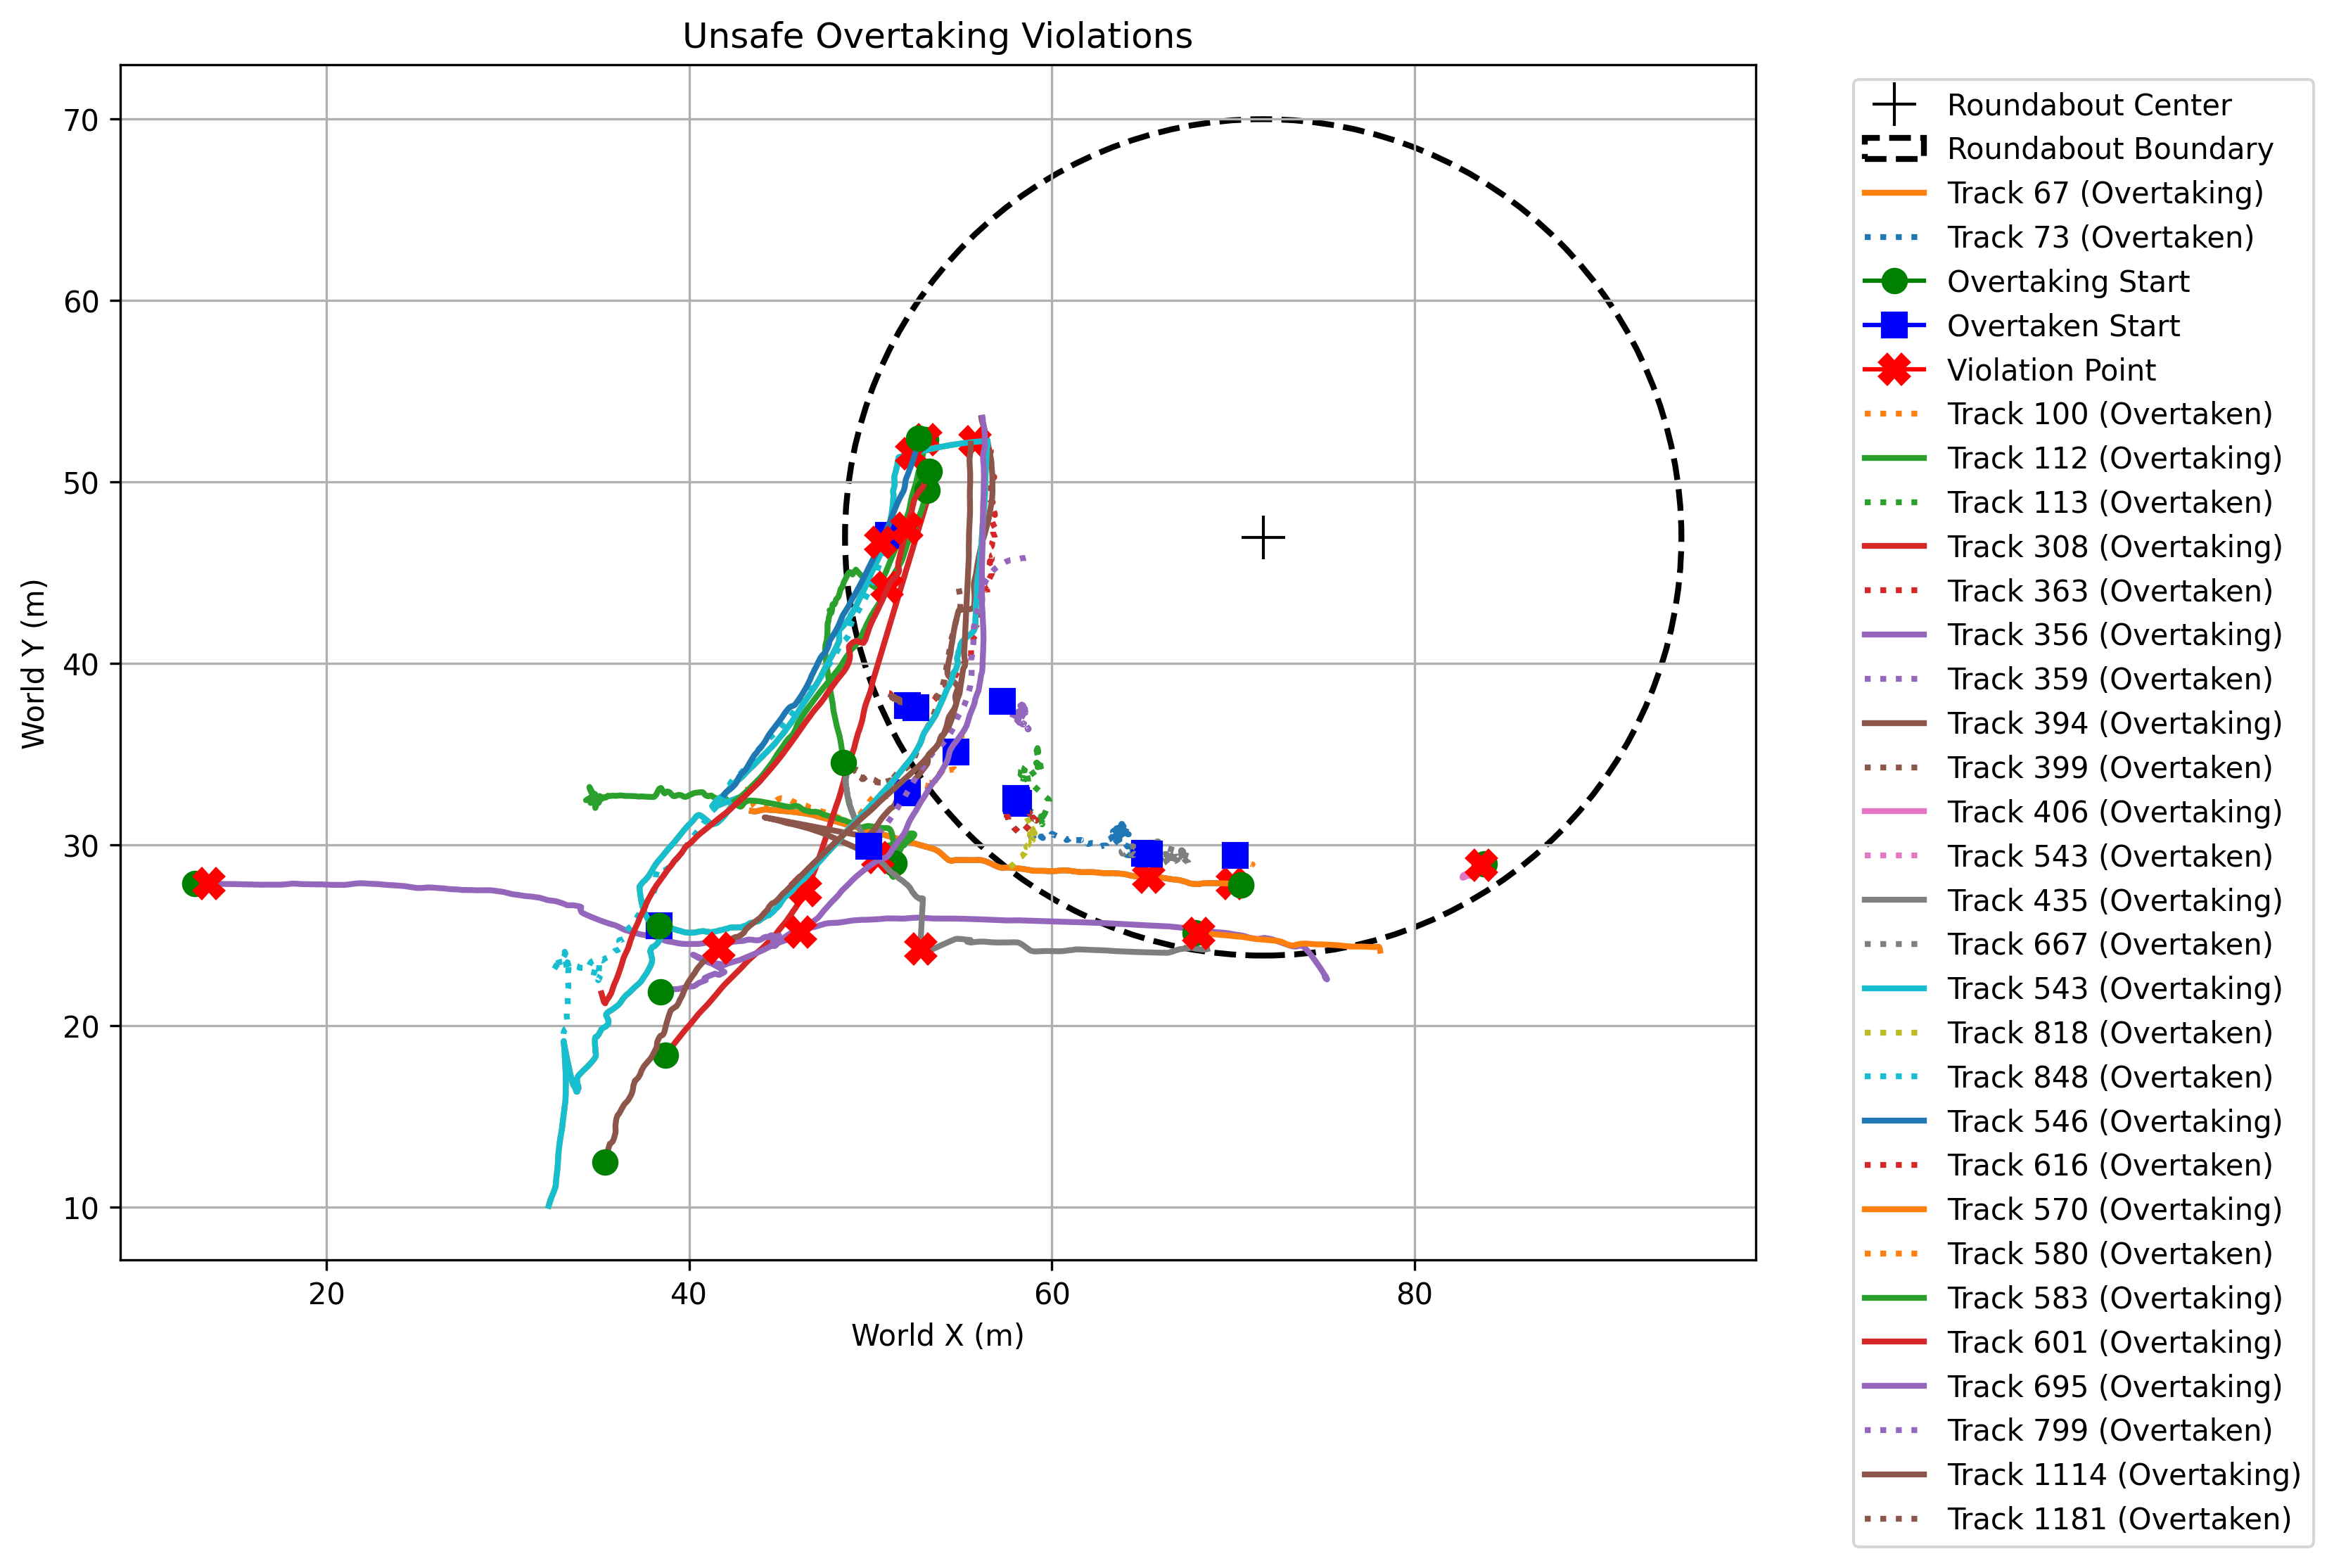
\includegraphics[width=0.55\textwidth]{../outputs/plots/overtaking.png}
\caption{Unsafe overtaking event identified by the safety rule framework. Trajectories of the overtaking vehicle (solid line) and overtaken vehicle (dotted line) are plotted alongside the exact violation trigger point (red marker).}
\label{fig:unsafe_overtaking_plot}
\end{figure}

% =========================================================================
\section{Rule 2: Tailgating Detection}
\label{sec:rule2}

\subsection{Intuition}
Tailgating occurs when a trailing follower vehicle follows a leading vehicle at an unsafe spatial gap while moving at active speed. In congested roundabout traffic, close following severely reduces reaction headway, elevating rear-end collision risk during sudden yields.

\subsection{Algorithm}
Vehicles within the same circulatory lane at frame $t$ are sorted by polar angle $\theta$. For consecutive follower--leader pairs $(i, j)$, the polar arc-length gap $d_{\text{arc\_ij}}$ is computed. A tailgating infraction is flagged if $d_{\text{arc\_ij}} < D_{\text{tailgate}} = 4.0$\,m and follower speed $v_i > V_{\text{min\_tailgate}} = 1.0$\,m/s.

\subsection{Mathematical Model}
The polar arc-length following distance along curved circulatory geometry is derived as:
\begin{equation}
    d_{\text{arc\_ij}}(t) = \left(\frac{r_i(t) + r_j(t)}{2}\right) \cdot \left[(\theta_j(t) - \theta_i(t)) \bmod 2\pi\right]
\end{equation}
where $r_i, \theta_i$ and $r_j, \theta_j$ denote the polar radii and angles of follower $i$ and leader $j$. The violation condition is:
\begin{equation}
    \mathcal{C}_{\text{tailgate}}(t) = \left( d_{\text{arc\_ij}}(t) < D_{\text{tailgate}} \right) \;\land\; \left( v_i(t) > V_{\text{min\_tailgate}} \right)
\end{equation}
The distance threshold $D_{\text{tailgate}} = 4.0$\,m corresponds to a 1.0-second headway at average roundabout speed ($\approx 4.0$\,m/s), while $v_i > 1.0$\,m/s prevents stationary queuing vehicles at entry points from triggering false positives.

\subsection{Pseudocode}
\begin{algorithm}[H]
\caption{Tailgating Detection Algorithm}
\label{alg:rule2}
\begin{algorithmic}[1]
\Require Trajectories $\mathcal{T}$, parameters $D_{\text{tailgate}} = 4.0$\,m, $V_{\text{min\_tailgate}} = 1.0$\,m/s
\Ensure Tailgating violation records $\mathcal{V}_{\text{tailgate}}$
\State $\mathcal{V}_{\text{tailgate}} \gets \emptyset$
\For{each frame $t$ and lane $L \in \{\text{Inner}, \text{Outer}\}$}
    \State Sort active vehicles in lane $L$ by ascending polar angle $\theta$
    \For{consecutive follower--leader pair $(i, j)$}
        \State Compute polar arc distance $d_{\text{arc\_ij}} \gets \frac{r_i + r_j}{2} \cdot \left[(\theta_j - \theta_i) \bmod 2\pi\right]$
        \If{$d_{\text{arc\_ij}} < D_{\text{tailgate}}$ \textbf{and} $v_i > V_{\text{min\_tailgate}}$}
            \State Record event $(t, \text{ID}_i, \text{ID}_j, L, d_{\text{arc\_ij}}, v_i)$ in $\mathcal{V}_{\text{tailgate}}$
        \EndIf
    \EndFor
\EndFor
\State \Return $\mathcal{V}_{\text{tailgate}}$
\end{algorithmic}
\end{algorithm}

% =========================================================================
\section{Rule 3: Wrong-Way Driving Detection}
\label{sec:rule3}

\subsection{Intuition}
Wrong-way driving occurs when a vehicle travels clockwise (opposite to mandatory counter-clockwise flow) inside the circulatory ring, creating critical head-on collision hazards.

\subsection{Algorithm}
Instantaneous angular velocity $\omega_i(t)$ is computed using continuous directional derivatives. A wrong-way violation is declared when $\omega_i(t) < \Omega_{\text{wrong}} = -0.1$\,rad/s and $v_i(t) \ge V_{\text{min\_wrong}} = 1.5$\,m/s continuously for $N_{\text{wrong}} \ge 45$ frames ($\approx 1.5$\,s).

\subsection{Mathematical Model}
Angular velocity is calculated via $\mathrm{atan2}$ phase-difference wrapping:
\begin{equation}
    \omega_i(t) = \mathrm{atan2}\!\left[\sin(\theta_i(t)-\theta_i(t{-}1)),\;\cos(\theta_i(t)-\theta_i(t{-}1))\right] \cdot f_{\text{ps}}
\end{equation}
The violation criterion requires sustained counter-directional motion:
\begin{equation}
    \sum_{m=0}^{N_{\text{wrong}}-1} \mathbb{1}\left[ \omega_i(t-m) < \Omega_{\text{wrong}} \;\land\; v_i(t-m) \ge V_{\text{min\_wrong}} \right] = N_{\text{wrong}}
\end{equation}
The 45-frame persistence requirement eliminates transient tracking noise, parking adjustments, and short evasive swerves.

\subsection{Pseudocode}
\begin{algorithm}[H]
\caption{Wrong-Way Driving Detection Algorithm}
\label{alg:rule3}
\begin{algorithmic}[1]
\Require Trajectories $\mathcal{T}$, parameters $\Omega_{\text{wrong}} = -0.1$\,rad/s, $V_{\text{min\_wrong}} = 1.5$\,m/s, $N_{\text{wrong}} = 45$
\Ensure Wrong-way violation records $\mathcal{V}_{\text{wrong}}$
\State $\mathcal{V}_{\text{wrong}} \gets \emptyset$
\For{each vehicle track $i$ inside ring $r_i \in [6.0, 14.0]$\,m}
    \State Initialize persistence counter $c_i \gets 0$
    \For{consecutive frames $t$}
        \State Compute $\omega_i(t) \gets \mathrm{atan2}(\sin(\theta_i(t)-\theta_i(t-1)), \cos(\theta_i(t)-\theta_i(t-1))) \cdot f_{\text{ps}}$
        \If{$\omega_i(t) < \Omega_{\text{wrong}}$ \textbf{and} $v_i(t) \ge V_{\text{min\_wrong}}$}
            \State $c_i \gets c_i + 1$
            \If{$c_i = N_{\text{wrong}}$}
                \State Record violation $(i, \text{class}_i, t - N_{\text{wrong}} + 1, t)$ in $\mathcal{V}_{\text{wrong}}$
            \EndIf
        \Else
            \State $c_i \gets 0$
        \EndIf
    \EndFor
\EndFor
\State \Return $\mathcal{V}_{\text{wrong}}$
\end{algorithmic}
\end{algorithm}

% =========================================================================
\section{Rule 4: Erratic Lane Weaving Detection}
\label{sec:rule4}

\subsection{Intuition}
Erratic lane weaving occurs when a vehicle executes rapid, un-signaled lateral transitions between inner and outer circulatory rings, destabilizing surrounding traffic flow.

\subsection{Algorithm}
Binary lane state $s_i(t) = \mathbb{1}[r_i(t) \ge R_{\text{boundary}}]$ where $R_{\text{boundary}} = 10.0$\,m is tracked per frame. An infraction is recorded when $K_{\text{weaving}} \ge 3$ boundary transitions occur within a rolling window of $W_{\text{weaving}} = 90$ frames ($\approx 3.0$\,s).

\subsection{Mathematical Model}
Given transition event set $\mathcal{E}_i = \{ t \mid s_i(t) \neq s_i(t{-}1) \land r_i(t) \in [6.0, 14.0] \}$, rolling window transition count is:
\begin{equation}
    n_{\text{weaving\_i}}(t) = | \{ t' \in \mathcal{E}_i \mid t - W_{\text{weaving}} + 1 \le t' \le t \} |
\end{equation}
The violation condition is:
\begin{equation}
    \mathcal{C}_{\text{weaving}}(t) = \left( n_{\text{weaving\_i}}(t) \ge K_{\text{weaving}} \right)
\end{equation}
Three lane transitions within 3 seconds distinguish reckless multi-lane weaving from standard single lane changes.

\subsection{Pseudocode}
\begin{algorithm}[H]
\caption{Erratic Lane Weaving Detection Algorithm}
\label{alg:rule4}
\begin{algorithmic}[1]
\Require Trajectories $\mathcal{T}$, parameters $R_{\text{boundary}} = 10.0$\,m, $W_{\text{weaving}} = 90$, $K_{\text{weaving}} = 3$
\Ensure Erratic lane weaving records $\mathcal{V}_{\text{weaving}}$
\State $\mathcal{V}_{\text{weaving}} \gets \emptyset$
\For{each vehicle track $i$ in trajectories $\mathcal{T}$}
    \State Extract transition set $\mathcal{E}_i \gets \{t \mid \mathbb{1}[r_i(t) \ge R_{\text{boundary}}] \neq \mathbb{1}[r_i(t-1) \ge R_{\text{boundary}}]\}$
    \For{each frame $t$}
        \State Compute window count $n_{\text{trans}} \gets |\{t' \in \mathcal{E}_i \mid t - W_{\text{weaving}} + 1 \le t' \le t\}|$
        \If{$n_{\text{trans}} \ge K_{\text{weaving}}$}
            \State Record event $(i, \text{class}_i, t - W_{\text{weaving}} + 1, t, n_{\text{trans}})$ in $\mathcal{V}_{\text{weaving}}$
        \EndIf
    \EndFor
\EndFor
\State \Return $\mathcal{V}_{\text{weaving}}$
\end{algorithmic}
\end{algorithm}

% =========================================================================
\section{Rule 5: Vehicle Stoppage Detection}
\label{sec:rule5}

\subsection{Intuition}
Vehicle stoppage occurs when a vehicle comes to an unauthorized complete stop inside an active circulatory lane, creating blockages for trailing traffic.

\subsection{Algorithm}
Deduplicated vehicle tracks ($d \ge 1.8$\,m / IoU $\le 0.20$) inside the circulatory ring are evaluated over a 90-frame retrospective window ($W_{\text{stoppage}} = 90$). A stoppage infraction is flagged when 90-frame displacement $\Delta d_{90\_i}(t) < D_{\text{stop}} = 1.0$\,m and rolling mean speed $\bar{v}_{90\_i}(t) < V_{\text{stop}} = 0.8$\,m/s.

\subsection{Mathematical Model}
Retrospective displacement and rolling mean velocity over window $W_{\text{stoppage}} = 90$ frames:
\begin{equation}
    \Delta d_{90\_i}(t) = \sqrt{(x_i(t)-x_i(t{-}90))^2 + (y_i(t)-y_i(t{-}90))^2}, \qquad
    \bar{v}_{90\_i}(t) = \frac{1}{90}\sum_{m=0}^{89} v_i(t-m)
\end{equation}
The violation condition is:
\begin{equation}
    \mathcal{C}_{\text{stoppage}}(t) = \left( \Delta d_{90\_i}(t) < D_{\text{stop}} \right) \;\land\; \left( \bar{v}_{90\_i}(t) < V_{\text{stop}} \right)
\end{equation}
Evaluating displacement over 3.0 seconds distinguishes prolonged vehicular blockages from temporary speed dips during yielding.

\subsection{Pseudocode}
\begin{algorithm}[H]
\caption{Vehicle Stoppage Detection Algorithm}
\label{alg:rule5}
\begin{algorithmic}[1]
\Require Trajectories $\mathcal{T}$, parameters $W_{\text{stoppage}} = 90$, $D_{\text{stop}} = 1.0$\,m, $V_{\text{stop}} = 0.8$\,m/s
\Ensure Vehicle stoppage records $\mathcal{V}_{\text{stop}}$
\State Apply deduplication filter on $\mathcal{T}$
\State $\mathcal{V}_{\text{stop}} \gets \emptyset$
\For{each vehicle track $i$ inside ring $r_i \in [6.0, 14.0]$\,m with duration $\ge W_{\text{stoppage}}$}
    \For{frame $t \ge W_{\text{stoppage}} - 1$}
        \State Compute $\Delta d_{90} \gets \sqrt{(x_i(t)-x_i(t-90))^2 + (y_i(t)-y_i(t-90))^2}$
        \State Compute $\bar{v}_{90} \gets \frac{1}{90}\sum_{m=0}^{89} v_i(t-m)$
        \If{$\Delta d_{90} < D_{\text{stop}}$ \textbf{and} $\bar{v}_{90} < V_{\text{stop}}$}
            \State Record event $(t, i, \mathrm{Lane}(r_i(t)), \Delta d_{90}, \bar{v}_{90})$ in $\mathcal{V}_{\text{stop}}$
        \EndIf
    \EndFor
\EndFor
\State \Return $\mathcal{V}_{\text{stop}}$
\end{algorithmic}
\end{algorithm}

\section{Rule Summary}

\begin{table}[H]
\centering
\small
\caption{Summary of safety rule conditions and output records (in priority evaluation order).}
\label{tab:rule_params}
\begin{tabularx}{\textwidth}{l X X}
\toprule
\textbf{Rule} & \textbf{Key Conditions} & \textbf{Output Record Fields} \\
\midrule
1. Unsafe Overtaking & sign flip of $\Delta_{ij}$, $d_{ij} \le 4.5$ m, $v_i \ge 0.8$ m/s & frame, overtaker ID, target ID \\
2. Tailgating      & $d_{\text{arc\_ij}} < 4.0$ m, $v_i > 1.0$ m/s & frame, follower ID, leader ID, lane, arc-distance \\
3. Wrong-Way       & $\omega_i < -0.1$ rad/s for $\ge 45$ frames, $v_i \ge 1.5$ m/s & track, class, start frame \\
4. Erratic Weaving & $\ge 3$ lane transitions in 90 frames & track, class, flagged-frame range \\
5. Vehicle Stoppage & $\Delta d_{90\_i} < 1.0$ m AND $\bar{v}_{90\_i} < 0.8$ m/s & frame, track, lane, displacement \\
\bottomrule
\end{tabularx}
\end{table}

The rule violation records exported by this stage are subsequently combined with manual dangerous-event annotations to form the ML training dataset (Chapter~\ref{chap:ml}).
\clearpage\thispagestyle{empty}\newpage

\chapter{Machine Learning Conflict Prediction Model}
\label{chap:ml}

\section{Problem Formulation}

While the deterministic safety rules described in Chapter~\ref{chap:safety} detect explicit, predefined rule violations (e.g., tailgating, wrong-way driving), complex traffic interactions often involve subtle kinematic patterns that do not violate any single rigid threshold yet still present significant safety risks. The machine learning component addresses this by learning a probabilistic danger score for arbitrary vehicle interaction pairs from labelled data.

To model vehicle interaction pairs without domain ambiguity, we introduce ML-specific notation replacing legacy terms:
\begin{itemize}
    \item \textbf{Aggressor Vehicle ($i$):} The primary vehicle being evaluated or classified (formerly referred to as ego or violating vehicle).
    \item \textbf{Suppressor Vehicle ($j$):} The relevant surrounding vehicle whose clearance or path is affected by the aggressor (formerly referred to as surrounding or lead vehicle).
\end{itemize}

The task is formulated as a regression problem: given the kinematic history of an Aggressor--Suppressor pair $(i, j)$ over a 75-frame retrospective window ($\approx 2.5$ seconds at 30 FPS), predict a continuous danger target score $y \in [0,1]$, where $y = 1$ denotes a critical near-collision interaction. The output score is mapped to five visual danger levels.

\section{Dataset Construction (Hybrid Labelling Strategy)}

The training dataset is constructed by combining two complementary sources of supervision:
\begin{enumerate}
    \item \textbf{Manually Annotated Dangerous Events (Tier 1):} Human expert inspection of drone video identified ground-truth dangerous interaction scenarios involving Aggressor vehicles and affected Suppressor vehicles.
    \item \textbf{Rule-Engine Violations (Tier 2):} Vehicle interaction pairs flagged by the five deterministic safety rules provide abundant, automatically extracted positive instances.
    \item \textbf{Background Safe Pairs (Tier 3):} Co-present vehicle pairs within a Euclidean distance range of $[2.0, 12.0]$ metres not flagged by Tier 1 or Tier 2 are sampled as safe instances.
\end{enumerate}

To reflect varying supervision confidence, Table~\ref{tab:weights} defines the target assignments and sample loss weights across tiers.

\begin{table}[H]
\centering
\caption{Training sample targets and assigned loss weights by tier and behavioral role.}
\label{tab:weights}
\begin{tabular}{lccc}
\toprule
\textbf{Source Tier} & \textbf{Role} & \textbf{Sample Targets ($y_i$)} & \textbf{Sample Weight ($w_i$)} \\
\midrule
Tier 1 -- Manual    & Aggressor Vehicle  & Dangerous (1.0) & 10.0 \\
Tier 1 -- Manual    & Suppressor Vehicle & Dangerous (1.0) & 3.0 \\
Tier 2 -- Automated & Aggressor Vehicle  & Dangerous (1.0) & 3.0 \\
Tier 2 -- Automated & Suppressor Vehicle & Dangerous (1.0) & 1.0 \\
Tier 3 -- Background& Safe Pair          & Safe (0.0)      & 1.0 \\
\bottomrule
\end{tabular}
\end{table}

The resulting training dataset contains \textbf{3,652 vehicle interaction pairs}: 960 from Tier 1, 866 from Tier 2, and 1,826 from Tier 3.

\section{Manual vs Automatic Annotation Comparison}

Table~\ref{tab:manual_vs_auto} compares manual expert annotation against automated safety-rule annotation across key operational dimensions.

\begin{table}[H]
\centering
\small
\caption{Comparative analysis of Manual Expert Annotation versus Automatic Safety-Rule Annotation.}
\label{tab:manual_vs_auto}
\begin{tabularx}{\textwidth}{l X X}
\toprule
\textbf{Aspect} & \textbf{Manual Expert Annotation} & \textbf{Automatic / Rule-Based Annotation} \\
\midrule
Supervision Focus & Complex, un-modeled evasive events & Predefined physical safety criteria \\
Scalability       & Labor-intensive for large videos & Highly scalable post-implementation \\
Consistency       & Subject to human annotator variability & 100\% deterministic under fixed thresholds \\
Coverage          & Captures novel driver interactions & Restricted to codified rule conditions \\
Annotation Cost   & High manual verification cost & Zero marginal cost across datasets \\
Reproducibility   & Dependent on subjective guidelines & Fully reproducible across arbitrary traffic \\
\bottomrule
\end{tabularx}
\end{table}

Combining manual annotations (high-precision ground truth) with rule-based outputs (high-volume weak supervision) creates a balanced training distribution that optimizes model robustness.

\section{Spatiotemporal Feature Engineering}

For each Aggressor--Suppressor pair $(i, j)$, kinematics are extracted over a 75-frame retrospective window sampled every 6th frame (13 discrete sample steps at offsets $\{0, 6, 12, \ldots, 72\}$). The 27-dimensional feature vector $\mathbf{f} \in \mathbb{R}^{27}$ comprises:
\begin{equation}
    \mathbf{f} = \bigl[d_{t_1}, \ldots, d_{t_{13}},\;\theta_{t_1}, \ldots, \theta_{t_{13}},\;v_{\text{rel}}\bigr]^\top
\end{equation}
where $d_{t_k}$ is inter-vehicle distance, $\theta_{t_k}$ is relative heading angle, and $v_{\text{rel}} = |v_i - v_j|$ is relative ground speed. No unsupported metrics (such as TTC or PET) are used.

\section{Model Selection Rationale: From Logistic Regression to Random Forest}

In early development stages, we evaluated linear classifiers such as Logistic Regression as a baseline. However, Logistic Regression assumes linear decision boundaries, which proved inadequate for traffic risk prediction due to two major limitations:
\begin{enumerate}
    \item \textbf{Non-Linear Kinematic Interactions:} Vehicle conflicts involve non-linear, non-monotonic feature combinations (e.g., a small inter-vehicle distance $d_{ij}$ accompanied by a sharp relative heading change $\theta_{rel}$ signifies a near-miss swerve, whereas the same distance at zero relative heading corresponds to safe parallel cruising). Linear models fail to capture such multi-variable interactions without exhaustive manual feature cross-products.
    \item \textbf{Continuous Probabilistic Grading for Multi-Level Risk:} Logistic Regression outputs binary decision probabilities that cluster aggressively near 0 or 1, making it difficult to establish well-separated intermediate risk tiers.
\end{enumerate}

To overcome these baseline limitations, we selected an ensemble \texttt{RandomForestRegressor} (\texttt{n\_estimators} = 300, \texttt{max\_depth} = 10) trained on the sample-weighted feature dataset. Random Forest decision trees naturally partition the 27-dimensional non-linear feature space without requiring explicit interaction terms. By formulating the target as continuous regression $y \in [0, 1]$ combined with out-of-fold Isotonic Calibration, the model outputs smooth, well-calibrated confidence scores. This continuous score distribution allows us to define precise, level-by-level thresholds ($[0, 0.30)$, $[0.30, 0.50)$, $[0.50, 0.65)$, $[0.65, 0.80)$, $[0.80, 1.00]$) mapping model confidence directly into five distinct visual danger classes.

\section{Probability Calibration and Video Inference}

Out-of-fold isotonic regression calibration (5-fold stratified CV) transforms raw ensemble outputs into true empirical probabilities representing danger risk $y \in [0, 1]$. During video inference, candidate Suppressor partners within an oriented spatial ellipse (15\,m ahead, 8\,m sideways) are evaluated per Aggressor vehicle. Stationary vehicles ($< 0.5$\,m/s over 6\,s) are excluded. Table~\ref{tab:danger_levels} defines the level-by-level confidence score mapping and visual rendering rules.

\begin{table}[H]
\centering
\caption{Danger level mapping, visual rendering colours, and temporal visual memory.}
\label{tab:danger_levels}
\begin{tabular}{l c c l}
\toprule
\textbf{Danger Level} & \textbf{Calibrated Score Range} & \textbf{Bounding Box Colour} & \textbf{Visual Memory} \\
\midrule
Level 0 -- Safe             & $[0.00, 0.30)$ & Unannotated & -- \\
Level 1 -- Nearly Safe      & $[0.30, 0.50)$ & Unannotated & -- \\
Level 2 -- Nearly Dangerous & $[0.50, 0.65)$ & Yellow      & 25 frames ($\approx 0.8$\,s) \\
Level 3 -- Dangerous        & $[0.65, 0.80)$ & Orange      & 50 frames ($\approx 1.7$\,s) \\
Level 4 -- Highly Dangerous & $[0.80, 1.00]$ & Red         & 75 frames ($\approx 2.5$\,s) \\
\bottomrule
\end{tabular}
\end{table}

Visual memory retains bounding-box highlights for a fixed frame duration, ensuring fleeting conflicts remain easily observable during manual video inspection.
\clearpage\thispagestyle{empty}\newpage

\chapter{Results and Evaluation}
\label{chap:results}

\section{Detection and Tracking Pipeline Performance}

The detection and tracking framework (SAHI + DINO detection backbone combined with ByteTrack and appearance feature prototype matching) was evaluated against manual CVAT bounding-box annotations across representative segments from the set of traffic videos.

\begin{table}[H]
\centering
\caption{Tracking evaluation metrics on the annotated video segment.}
\label{tab:tracking_metrics}
\begin{tabular}{lccccc}
\toprule
\textbf{Class} & \textbf{MOTA} & \textbf{IDF1} & \textbf{Precision} & \textbf{Recall} & \textbf{F1-Score} \\
\midrule
\textbf{Overall} & 55.81\% & 73.27\% & 0.855 & 0.673 & 0.753 \\
Person           & 60.04\% & 77.76\% & 0.809 & 0.786 & 0.797 \\
Car              & 40.02\% & 61.66\% & 0.848 & 0.488 & 0.619 \\
Motorcycle       &  5.46\% & 47.67\% & 0.532 & 0.456 & 0.491 \\
\bottomrule
\end{tabular}
\end{table}

Key observations:
\begin{itemize}
    \item The overall IDF1 score of 73.27\% verifies that the tracking pipeline maintains stable identity preservation across severe occlusions, providing reliable metric trajectories for downstream safety evaluation.
    \item Pedestrian tracking achieves the highest performance (IDF1 77.76\%), benefiting from distinctive appearance features and minimal mutual occlusion compared to motorized vehicles.
    \item Motorcycle tracking yields lower MOTA (5.46\%) and IDF1 (47.67\%), caused by visual similarity, small pixel surface area, and dense clustering typical of Indian roundabout traffic.
\end{itemize}

\section{Safety Rule Engine Evaluation}

The deterministic safety rules were evaluated on 600 vehicle-level observations captured from 1-minute video footage recorded at 30 FPS. Table~\ref{tab:safety_rule_full_eval} reports the complete confusion-matrix counts and derived performance metrics for Wrong-Way Driving Detection and Tailgating Detection.

\begin{table}[H]
\centering
\caption{Safety rule evaluation metrics for 1-minute video footage ($\approx 600$ observations).}
\label{tab:safety_rule_full_eval}
\begin{tabular}{lcc}
\toprule
\textbf{Metric} & \textbf{Wrong-Way Detection} & \textbf{Tailgating Detection} \\
\midrule
True Positive (TP) & 18 & 17 \\
False Positive (FP) & 6 & 19 \\
False Negative (FN) & 12 & 9 \\
True Negative (TN) & 564 & 555 \\
\midrule
Total Observations & 600 & 600 \\
Actual Positives ($\text{TP}+\text{FN}$) & 30 & 26 \\
Predicted Positives ($\text{TP}+\text{FP}$) & 24 & 36 \\
Actual Negatives ($\text{TN}+\text{FP}$) & 570 & 574 \\
\midrule
\textbf{Precision} & \textbf{75.00\%} & \textbf{47.22\%} \\
\textbf{Recall / Sensitivity} & \textbf{60.00\%} & \textbf{65.38\%} \\
\textbf{F1-Score} & \textbf{66.67\%} & \textbf{54.84\%} \\
Accuracy & 97.00\% & 95.33\% \\
Specificity & 98.95\% & 96.69\% \\
\textbf{False Positive Rate (FPR)} & \textbf{1.05\%} & \textbf{3.31\%} \\
\textbf{False Negative Rate (FNR)} & \textbf{40.00\%} & \textbf{34.62\%} \\
Negative Predictive Value (NPV) & 97.92\% & 98.40\% \\
Balanced Accuracy & 79.47\% & 81.04\% \\
Jaccard / IoU & 50.00\% & 37.78\% \\
Matthews Correlation Coefficient (MCC) & 0.656 & 0.532 \\
\bottomrule
\end{tabular}
\end{table}

\subsection{Analysis of Primary Metrics}

\paragraph{Class Imbalance and Accuracy Interpretation.}
Because safety infractions constitute a minor fraction of overall traffic flow ($30$ actual wrong-way events and $26$ actual tailgating events out of 600 observations), the dataset exhibits class imbalance. Consequently, global Accuracy ($97.00\%$ for Wrong-Way and $95.33\%$ for Tailgating) is heavily influenced by the large number of True Negatives. Performance evaluation therefore focuses primarily on Precision, Recall, F1-Score, FPR, and FNR.

\paragraph{Precision.}
Wrong-Way Detection achieves a significantly higher Precision of \textbf{75.00\%} compared to \textbf{47.22\%} for Tailgating Detection. When the system flags a wrong-way entry, three out of four alerts correspond to actual counter-directional violations, whereas tailgating alerts generate more frequent false positives due to transient decelerations in crowded lanes.

\paragraph{Recall and Sensitivity.}
Tailgating Detection yields a slightly higher Recall of \textbf{65.38\%} (17 out of 26 events detected) than Wrong-Way Detection at \textbf{60.00\%} (18 out of 30 events detected). This indicates that tailgating detection captures a slightly greater proportion of actual physical follow-distance breaches.

\paragraph{F1-Score and Overall Trade-Off.}
The F1-Score balances Precision and Recall:
\begin{equation}
    \text{F1} = 2 \times \frac{\text{Precision} \times \text{Recall}}{\text{Precision} + \text{Recall}}
\end{equation}
Wrong-Way Detection achieves a superior overall F1-Score of \textbf{66.67\%} compared to \textbf{54.84\%} for Tailgating Detection. Furthermore, Wrong-Way Detection maintains a very low False Positive Rate ($\text{FPR} = 1.05\%$), minimizing unnecessary driver alerts, whereas Tailgating Detection exhibits a higher false alarm rate ($\text{FPR} = 3.31\%$). Overall, Wrong-Way Detection demonstrates the stronger precision--recall balance, while Tailgating Detection offers higher sensitivity at the expense of increased false alarms.

In addition to rule evaluation, quantitative recall was evaluated for the Unsafe Overtaking rule against 38 manually annotated overtaking events, detecting 22 pairs (\textbf{57.9\% recall}), with unflagged events primarily corresponding to gradual maneuvers extending beyond the 10-frame window.

\section{Machine Learning Conflict Prediction Results}

The Random Forest conflict prediction model operates within the end-to-end project pipeline:
\begin{align*}
&\text{Set of Traffic Videos} \rightarrow \text{SAHI + DINO Detection} \rightarrow \text{ByteTrack Tracking} \\
&\rightarrow \text{Metric Trajectories} \rightarrow \text{Safety Rule Engine} \\
&\rightarrow \text{Hybrid Dataset (Rules + Annotations)} \rightarrow \text{Random Forest Model}
\end{align*}

The model was evaluated using two validation strategies:
\begin{enumerate}
    \item \textbf{5-Fold Stratified Cross-Validation (80-20 Split):} The dataset is partitioned into 5 folds with an 80\% training and 20\% testing proportion per fold.
    \item \textbf{Stratified Shuffle Split (70-30 Split):} Configured explicitly as a 70\% training and 30\% testing split across 5 independent iterations.
\end{enumerate}

Table~\ref{tab:ml_validation_comparison} presents the experimental results across both validation configurations.

\begin{table}[H]
\centering
\caption{ML model experimental results under 80-20 5-Fold Cross-Validation and 70-30 Stratified Shuffle Split.}
\label{tab:ml_validation_comparison}
\begin{tabular}{lccc}
\toprule
\textbf{Metric} & \textbf{80-20 Split (5-Fold CV)} & \textbf{70-30 Split (Shuffle Split)} & \textbf{Change} \\
\midrule
Accuracy (ACC) & 94.11\% $\pm$ 1.13\% & 93.43\% $\pm$ 1.33\% & -0.68\% \\
Precision      & 97.84\% $\pm$ 0.45\% & 97.81\% $\pm$ 0.32\% & -0.03\% \\
Recall         & 95.41\% $\pm$ 1.26\% & 94.64\% $\pm$ 1.29\% & -0.77\% \\
F1 Score       & 0.9660 $\pm$ 0.0068  & 0.9619 $\pm$ 0.0079  & -0.0041 \\
\bottomrule
\end{tabular}
\end{table}

\subsection{Expanded Academic Interpretation}

\paragraph{Accuracy.}
The Random Forest model achieves an Accuracy of $94.11\% \pm 1.13\%$ under the 80-20 cross-validation setting and $93.43\% \pm 1.33\%$ under the 70-30 shuffle-split setting. The relatively small decrease of 0.68 percentage points indicates that overall classification performance remains consistent when the training/testing proportion is changed.

\paragraph{Precision.}
Precision remains consistently high across both validation strategies ($97.84\% \pm 0.45\%$ under 80-20 CV vs $97.81\% \pm 0.32\%$ under 70-30 Shuffle Split). The high precision indicates a low proportion of false-positive classifications within the evaluated test partitions. High precision is particularly valuable in traffic-safety analysis because excessive false-positive alerts can reduce the usefulness of an automated safety-monitoring system and potentially cause alert fatigue among safety operators.

\paragraph{Recall.}
Recall represents the proportion of true dangerous traffic interactions successfully identified by the model ($95.41\% \pm 1.26\%$ under 80-20 CV vs $94.64\% \pm 1.29\%$ under 70-30 Shuffle Split). Recall is slightly lower than precision, indicating that a small fraction of dangerous instances remain difficult for the model to identify. This distinction is important in safety analysis because false negatives correspond to dangerous traffic situations that remain undetected by the classifier.

\paragraph{F1 Score.}
The model achieves high F1 scores of $0.9660 \pm 0.0068$ under 80-20 CV and $0.9619 \pm 0.0079$ under 70-30 Shuffle Split, demonstrating a strong harmonic balance between precision and recall. The decrease of only 0.0041 indicates that the model maintains a similar precision-recall balance across both evaluated validation configurations.

\paragraph{Evaluation of Training Set Size Sensitivity (80-20 vs 70-30 Difference).}
Comparing the 80-20 cross-validation and 70-30 shuffle-split results reveals minimal performance shifts: Accuracy changes by $-0.68$ percentage points, Precision by $-0.03$ percentage points, Recall by $-0.77$ percentage points, and F1 Score by $-0.0041$. In particular, precision changes by only 0.03 percentage points and F1 score by only 0.0041. The limited performance degradation observed when reducing the training proportion suggests that the model has learned stable patterns from the available traffic features and does not exhibit substantial sensitivity to the evaluated change in training-set size.

\paragraph{Variability and Standard Deviation.}
The experimental results are reported as Mean $\pm$ Standard Deviation across five evaluated folds/iterations, where the mean represents average performance and the standard deviation reflects performance variation across evaluations. The reported standard deviations are relatively small: Accuracy varies by approximately 1.1--1.3 percentage points, Precision remains below 0.5 percentage points, Recall varies by approximately 1.3 percentage points, and F1 score variation remains below 0.01. The relatively low variation across the evaluated splits provides evidence of stable model performance under the tested validation configurations.

\paragraph{Probability Calibration Results.}
In addition to classification performance, probability calibration was evaluated using the Brier Score. Out-of-fold isotonic calibration improved the Brier Score from 0.0935 (uncalibrated) to 0.0847 (calibrated), representing a 9.4\% relative improvement and verifying that calibrated outputs closely track empirical collision probabilities.
\clearpage\thispagestyle{empty}\newpage

\chapter{Discussion, Limitations, and Future Work}
\label{chap:discussion}

\section{Discussion of Key Findings}

The experimental results validate the core hypothesis of this thesis: an integrated pipeline combining high-recall
detection, metric coordinate mapping, rule-based reasoning, and calibrated machine learning can automatically
characterize traffic safety in dense overhead video without specialized ground sensors.

Key insights include:
\begin{itemize}
    \item \textbf{SAHI + DINO Detection:} Slicing aerial imagery prevents downsampling loss for small vehicles.
          The contrastive denoising head in DINO stabilizes confidence across adjacent tiles, enabling cleaner
          box fusion and reducing track initialization errors.
    \item \textbf{Physical Calibration via Laser Measurement:} Grounding the scale factor in a physical field measurement
          (7.0 m lane width measured with a laser distance meter) establishes a direct physical meaning for spatial
          thresholds across all downstream rules and ML models.
    \item \textbf{Hybrid Rule-ML Pipeline:} Deterministic safety rules provide clear physical interpretations for
          specific infractions while generating high-volume weak supervision. Combining rule outputs with manually
          annotated ground-truth conflicts allows the ML model to learn complex, non-linear interaction dynamics.
\end{itemize}

\section{Limitations}

\begin{enumerate}
    \item \textbf{Uniform Scale Factor Assumption:} Converting image coordinates using a uniform scale factor
          ($s \approx 0.0824$ m/px) assumes a strictly nadir camera perspective. Small camera tilt angles cause slight
          scale distortion near frame borders.
    \item \textbf{Motorcycle Tracking Identity Shifts:} Heavy motorcycle clustering leads to identity switches (IDF1 47.67\%)
          due to high visual similarity and frequent mutual occlusions.
    \item \textbf{Single-Intersection Validation:} All evaluation was performed on video captured at one specific
          roundabout. Broad generalizability across diverse intersection geometries remains to be benchmarked.
\end{enumerate}

\section{Future Work}

\begin{itemize}
    \item \textbf{Multi-Point Homography Calibration:} Incorporate a full 4-point planar homography matrix using ground control
          points to eliminate tilt-induced scale variation across the image.
    \item \textbf{Graph Neural Network Conflict Models:} Model vehicle interactions as dynamic spatial-temporal graphs
          to capture multi-vehicle group interactions beyond pairwise relationships.
    \item \textbf{Multi-Site Benchmark Datasets:} Expand drone video acquisition to multiple heterogeneous unsignalized
          intersections across different weather and lighting conditions.
\end{itemize}
\clearpage\thispagestyle{empty}\newpage

\chapter{Conclusion}
\label{chap:conclusion}

This thesis presented a comprehensive end-to-end system for automated traffic safety analysis from aerial drone footage of an unsignalized Indian roundabout intersection.

The primary contributions and conclusions are summarized below:
\begin{enumerate}
    \item \textbf{High-Recall Aerial Detection and Tracking:} Combining SAHI sliced inference with a DINO-style RT-DETRv2-X backbone
          and an appearance-augmented ByteTrack algorithm addresses the challenges of small object scale and dense vehicle clustering,
          achieving an overall tracking IDF1 of 73.27\%.
    \item \textbf{Ground-Truthed World Coordinate Mapping:} Performing direct physical measurements at the intersection using a laser distance
          meter established an empirical scale calibration ($s \approx 0.0824$ m/px), allowing pixel trajectories to be transformed into
          metrically accurate spatial representations.
    \item \textbf{Deterministic Safety Rule Engine:} Five domain-specific safety rules (tailgating, wrong-way driving, erratic lane weaving,
          unsafe overtaking, and vehicle stoppage) were formulated and evaluated in world coordinates, providing interpretable safety metrics
          and automated infraction records.
    \item \textbf{Hybrid Machine Learning Conflict Predictor:} Combining rule-engine violation outputs with manually annotated dangerous traffic
          events produced a balanced 3,652-pair training dataset. A calibrated Random Forest regressor utilizing 27-dimensional spatiotemporal
          kinematic features achieved 96.60\% cross-validation F1-score under 80-20 CV (and 96.19\% under 70-30 shuffle split), demonstrating consistent model performance across data partitioning strategies, along with a calibrated Brier score of 0.0847.
\end{enumerate}

The resulting framework demonstrates that drone video, combined with physical field calibration, rule-based reasoning, and machine learning,
can provide automated, objective, and detailed traffic safety intelligence for complex unsignalized intersections.
\clearpage\thispagestyle{empty}\newpage

%% ---- Bibliography -----------------------------------------
\fancyhead[LE]{\bfseries\small{Bibliography}}
\fancyhead[RO]{\bfseries\small{Bibliography}}
\addcontentsline{toc}{chapter}{Bibliography}
\bibliographystyle{IEEEtran}
\bibliography{chapters/references/refs}

\end{document}